\section{Brintatomet}
Den radiale Schrödingerligningen er givet ved \cite[s. 140]{griffiths}
%
\begin{align}
    \frac{-\hbar^{2}}{2m}\diff[2]{u(r)}{r} + \overbrace{\left( - \frac{e^{2}}{4\pi\epsilon_{0}r} + \frac{\hbar^{2}}{2m}\frac{l(l+1)}{r^{2}} \right)}^{V_{\text{eff}}} u(r) &  = Eu(r).
\end{align}
%
hvor $V_{\text{eff}}$ er en sum af det velkendte Coulomb potentiale og et led tilhørende den ekstra, rotationelle frihedsgrad. Dermed har vi en differentialligning på samme form som tidligere.

Fra \cite{griffiths} kendes bohrradien, $a_{0}$ og rydbergenergien $\mathrm{Ry}$ til følgende værdier;
\begin{align}
    a_{0} = \frac{\hbar^{2}}{2m} {\left(\frac{e^{2}}{4\pi\epsilon_{0}} \right) \quad \text{og} \quad \mathrm{Ry} = \frac{m}{2\hbar^{2}}\left(\frac{e^{2}}{4\pi\epsilon_0} \right)}^{2}.
    \label{eq:konstanter}
\end{align}
%
Da energien kan vælges at skrives som et produkt af rydbergenergien og en konstant $\varepsilon \in \mathbb{R}$ således at $E=-\varepsilon \mathrm{Ry}$, og idet man kan genkende, at ${a_{0}}^{2}\mathrm{Ry} = \frac{\hbar^{2}}{2m}$, samt at $2a_{0}\mathrm{Ry} = \frac{e^{2}}{4\pi\epsilon_{0}}$, kan det skrives at,
\begin{align}
    k(r) = & \frac{1}{\hbar} \sqrt{2m\left( E - V_{\text{eff}} \right)}\\
    = & \sqrt{\frac{1}{a_{0}^{2}\mathrm{\mathrm{Ry}}} \left( E + \frac{e^{2}}{4\pi\epsilon_{0}r} - \frac{\hbar^{2}}{2m}\frac{l(l+1)}{r^{2}} \right)}\\
    = & \sqrt{\frac{1}{a_{0}^{2}\mathrm{Ry}} \left( (-\varepsilon \mathrm{Ry}) + \frac{2a_{0}\mathrm{Ry}}{r} - a_{0}^{2}\mathrm{Ry}\frac{l(l+1)}{r^{2}} \right)}\\
    = & \frac{1}{r} \sqrt{\frac{1}{a_{0}^{2}{Ry}} \left( (-\varepsilon \mathrm{Ry})r^{2} + 2a_{0}\mathrm{Ry} r - a_{0}^{2}\mathrm{Ry} l(l+1) \right)}.
\end{align}
Nu kan $\frac{1}{a_0}$ trækkes udenfor kvadratroden, og ved at gange $\mathrm{Ry}$ ind i parantesen vil man få
\begin{align}
    k(r) = & \frac{1}{a_0} \frac{1}{r} \sqrt{-\varepsilon r^2 + 2a_0r - a_0^2l(l+1)}, \\
    = & \frac{\sqrt{\varepsilon}}{a_0} \frac{1}{r} \sqrt{r^2 - \frac{2a_0}{\varepsilon}r + \frac{a_0^2}{\varepsilon}l(l+1)}.
\end{align}
Det indre af kvadratroden genkendes at være på formen $x^2 -x(a+b) + ab = (x-a)(x-b)$. Det er af interesse at bestemme $a$ og $b$ til at være de klassiske vendepunkter, da $k(a) = 0 = k(b)$. Da faktoren udenfor kvadratroden ikke er $0$, må det indre af kvadratroden være $0$.
%
\begin{align}
    r^2 - \frac{2a_0}{\varepsilon}r + \frac{a_0^2}{\varepsilon}l(l+1) = 0.
\end{align}
Dette har løsninger ved
\begin{align}
  r = \frac{\frac{2a_0}{\varepsilon} \pm \sqrt{\frac{4a_0^2}{\varepsilon^2} - \frac{4a_0^2}{\varepsilon}l(l+1)   }  }{2}
  = \frac{a_0}{\varepsilon}\left[1 \pm \sqrt{1-\varepsilon l(l+1)}\right].
\end{align}
Herved bliver de klassiske vendepunkter
\begin{align}
    a =  \frac{a_0}{\varepsilon}\Bigl[1-\sqrt{1-\varepsilon l(l+1)}  \Bigr],\quad \text{og} \quad b = \frac{a_0}{\varepsilon}\Bigl[1+\sqrt{1-\varepsilon l(l+1)}  \Bigr].
\end{align}
For at det nu skal passe i vores udtryk for $k(r)$ tjekkes det om
\begin{align}
    a+b = \frac{2a_0}{\varepsilon} \quad \text{og} \quad  ab  = \frac{a_0^2}{\varepsilon} l(l+1).
\end{align}
$a+b$ leddet er oplagt, mens $ab$ leddet bliver
\begin{align}
  ab = & \frac{a_0^2}{\varepsilon^2}\Bigl(1-\sqrt{1-\varepsilon l(l+1)} \Bigr)\Bigl(1+\sqrt{1-\varepsilon l(l+1)} \Bigr)\\
     = & \frac{a_0^2}{\varepsilon^2}\Bigl(1-(1-\varepsilon l(l+1)) \Bigr) =  \frac{a_0^2}{\varepsilon^2} \varepsilon l(l+1)
     = \frac{a_0^2}{\varepsilon} l(l+1).
\end{align}
%
\fxnote{HERFRA}
Det stemmer overens, hvorfor der arbejdes videre med disse værdierne.
\begin{align}
    k(r) = & \frac{p(r)}{\hbar} = \frac{\sqrt{\varepsilon}}{a_0}\frac{1}{r}\sqrt{(r-a)(r-b)}.
\end{align}
Nu kan vi altså integrere fra $a$ til $b$, som er de klassiske vendepunkter og bruge \cref{eq:kvantiDone}.
\begin{equation}
  \int_{a}^{b}k(r)dr = \frac{\sqrt{\varepsilon}}{a_0} \Bigl[\frac{\pi}{2}(\sqrt{b}-\sqrt{a})^2  \Bigr]
\end{equation}
Her er det brugt at
\begin{equation}
  \int_{\alpha}^{\beta}\frac{1}{u}\sqrt{(u-\alpha)(u-\beta)}du = \frac{\pi}{2}(\sqrt{\beta}-\sqrt{\alpha})^2
\end{equation}
Herfra følger det at
\begin{align}
  n' = & \frac{\sqrt{\varepsilon}}{2a_0}(\sqrt{b}-\sqrt{a})^2 = \frac{\sqrt{\varepsilon}}{2a_0}(b+a-2\sqrt{ab})\\
     = & \frac{\sqrt{\varepsilon}}{2a_0}\Bigl(\frac{2a_0}{\varepsilon}-2a_0\sqrt{\frac{1}{\varepsilon}l(l+1)}\Bigr)\\
     = & \frac{1}{\sqrt{\varepsilon}} -l(l+1)
\end{align}
Herfra finder vi $\varepsilon$ til at være
\begin{equation}
  \varepsilon = \frac{1}{\Bigl[n'+l(l+1)  \Bigr]^2}
\end{equation}
Og da $E = -\varepsilon Ry$, så kan vi skrives
\begin{equation}
  E_{n',l} = \frac{-Ry}{\Bigl[n'+l(l+1)  \Bigr]^2}
\end{equation}

Nu kigger vi på den asymptotiske form for bølgefunktionerne ved store $r$.
I det eksakte tilfælde er de på formen
\begin{equation}
  R_{nl}(r) \sim \left(\frac{r}{a_0}\right)^{n-1}e^{-r/na_0}
  \label{eq:eksatR}
\end{equation}

For at finde dem i WKB tilfældet kigges først på formen af en sådan bølgefunktion. Det kan vises at den er på formen %TODO find formen her
\begin{equation}
  u(r) \sim exp\Bigl[-\int_{a_0}^{r}k(r')dr'\Bigr]
\end{equation}
Først kigges der på $k(r)$ da vi gerne vil lave en rækkeudvikling da vi kun kigger på meget store $r$.
Vi har altså at
\begin{equation}
  k(r) = \frac{\sqrt{\varepsilon}}{a_0}\frac{1}{r}\sqrt{(r-a)(r-b)}
\end{equation}
Her lader vi $\frac{1}{r}$ gå ind under kvadratroden og vi får
\begin{align}
  k(r) = & \frac{\sqrt{\varepsilon}}{a_0}\sqrt{(1-\frac{a}{r})(1-\frac{b}{r})} = \frac{\sqrt{\varepsilon}}{a_0}\sqrt{1-\frac{a+b}{r}+\frac{ab}{r^2}}
\end{align}
Her beholder vi kun til første orden og vi får altså noget som vi kan rækkeudvikle ved den sædvanelige kvadratrods række.
\begin{align}
  k(r) \approx & \frac{\sqrt{\varepsilon}}{a_0}\sqrt{1-\frac{a+b}{r}}\\
       = & \frac{\sqrt{\varepsilon}}{a_0}(1-\frac{1}{2}\frac{a+b}{r})
\end{align}
Husker vi på $a+b = \frac{2a_0}{\varepsilon}$ så får vi
\begin{equation}
  k(r) = \frac{\sqrt{\varepsilon}}{a_0}-\frac{1}{\sqrt{\varepsilon}r}
\end{equation}
\\
Kigger vi da på integralet har vi at
\begin{align}
  \int_{a_0}^{r}k(r')dr' = & \frac{\sqrt{\varepsilon}}{a_0}(r-a_0) - \frac{1}{\sqrt{\varepsilon}}\left(\ln{r}-\ln{a_0}\right)\\
  = & \frac{\sqrt{\varepsilon}}{a_0}(r-a_0) - \ln{((\frac{r}{a_0})^{\frac{1}{\sqrt{\varepsilon}}})}
\end{align}
%
Så nu kan vi altså skrive vores $u(r)$ op som
\begin{align}
  u(r) \sim & \exp\left[-\frac{\sqrt{\varepsilon}}{a_0}(r-a_0) + \ln{((\frac{r}{a_0})^{\frac{1}{\sqrt{\varepsilon}}})}\right]\\
        = & \exp\left[-\frac{\sqrt{\varepsilon}}{a_0}(r-a_0)\right] + (\frac{r}{a_0})^{\frac{1}{\sqrt{\varepsilon}}}\\
        = & \exp\left[\sqrt{\varepsilon}(1-\frac{r}{a_0})\right] + (\frac{r}{a_0})^{\frac{1}{\sqrt{\varepsilon}}}
\end{align}
Nu bruges det blot at
\begin{equation}
  \varepsilon = \frac{1}{\left[n'+\sqrt{l(l+1)}\right]^2}
\end{equation}
Og det giver os altså at
\begin{equation}
  u(r) \sim {\left(\frac{r}{a_0}\right)}^{\left[n'+\sqrt{l(l+1)}\right]} e^{\left[\frac{1-\frac{r}{a_0}}{n'+\sqrt{l(l+1)}}\right]}
\end{equation}
Derved bliver $R(r) = u(r)/r$
\begin{equation}
  R(r) = \frac{1}{a_0}{\left(\frac{r}{a_0}\right)}^{\left[n'-1+\sqrt{l(l+1)}\right]} e^{\left[\frac{1-\frac{r}{a_0}}{n'+\sqrt{l(l+1)}}\right]}
  \label{eq:rAfR}
\end{equation}
Dette giver anledning til en sammenligning mellem \cref{eq:eksatR} og \cref{eq:rAfR}. Det ses at vi i begge udtryk har to led: et polynomielt led og et eksponentielt led. WKB approksimationen har dog taget højde for kvantetallet $l$ hvilket den eksakte løsning ikke har, hvilket ses

\begin{figure}[h!]
    \centering
    \begin{subfigure}{0.45\textwidth}
        \centering
        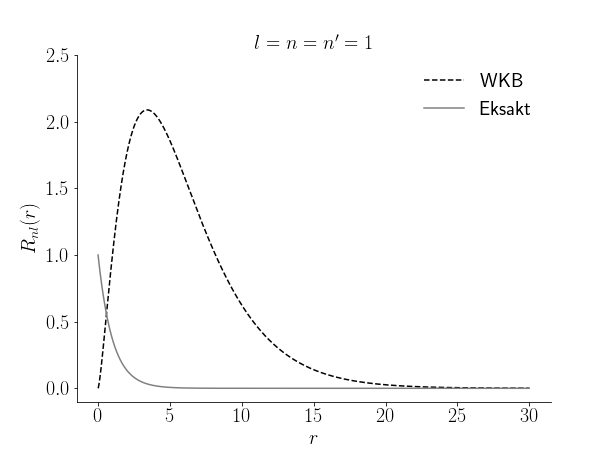
\includegraphics[width=\columnwidth]{sammenligning.png}
        \caption{Hydrogen}
        \label{fig:hydrogen}
    \end{subfigure}
    \begin{subfigure}{0.45\textwidth}
        \centering
        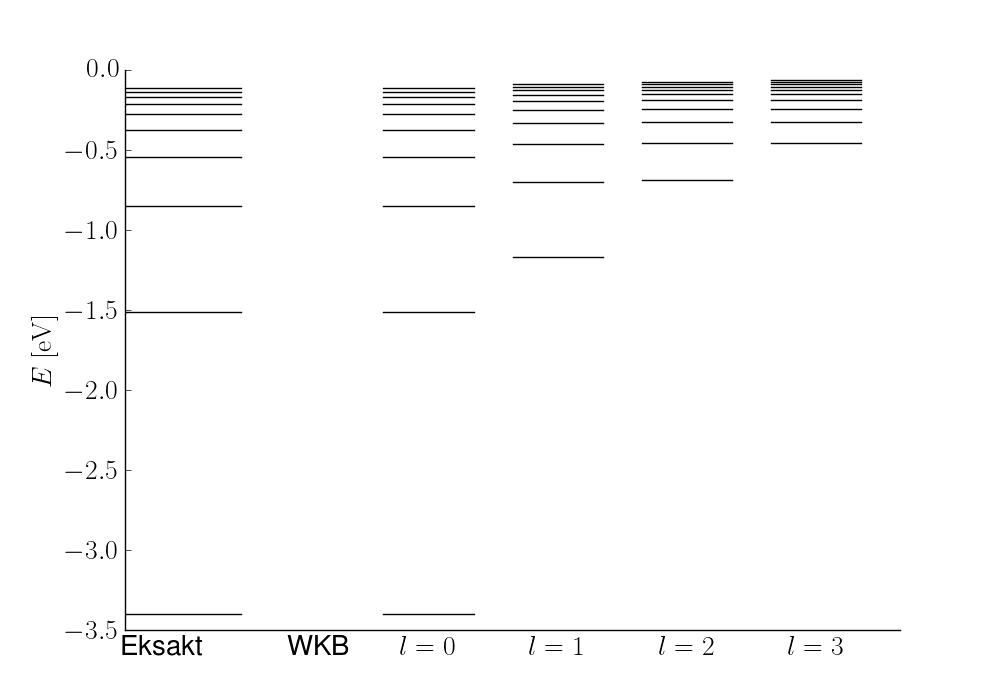
\includegraphics[width=\columnwidth]{energyPlot}
        \caption{Hydrogen}
        \label{fig:sammenlign}
    \end{subfigure}
    \caption{2 figurer}
    \label{storfig}
\end{figure}


%
